% begin module limits-infinite-def
\begin{frame}[t]
\begin{definition}[Infinite Limit]
Let $f$ be a function defined on both sides of $a$, except perhaps at $a$.  Then
\[
\lim_{x\rightarrow a}f(x) = \infty 
\]
means the values of $f(x)$ can be made arbitrarily large by taking $x$ sufficiently close to $a$, but not equal to $a$.
\end{definition}
\begin{columns}[c]
\column{.4\textwidth}
\psset{xunit=0.15cm, yunit=0.15cm}
\begin{pspicture}(-10,-7)(26,20)
%\psframe*[linecolor=white](-5,-1)(5,5) 
\psaxes[labels=none, ticks=none]{<->}(0,0)(-10,-3)(25,15)
\psplot[linecolor=red, plotpoints=1000]{1.39}{25}{x 1 x -1 add 2 exp div mul 0.8 mul x x mul 1 x -1 add 2 exp div mul 1.05 mul add 1 x -1 add 2 exp div 0.15 mul add -2 add }
\psplot[linecolor=red, plotpoints=1000]{-10}{0.75}{x 1 x -1 add 2 exp div mul 0.8 mul x x mul 1 x -1 add 2 exp div mul 1.05 mul add 1 x -1 add 2 exp div 0.15 mul add -2 add }
\psline[linestyle=dotted](1, -7)(1, 20)
\rput[l](1.5,-5){$x=a$}
\rput(8,3.5){$y=f(x)$}
\end{pspicture}%
%\ 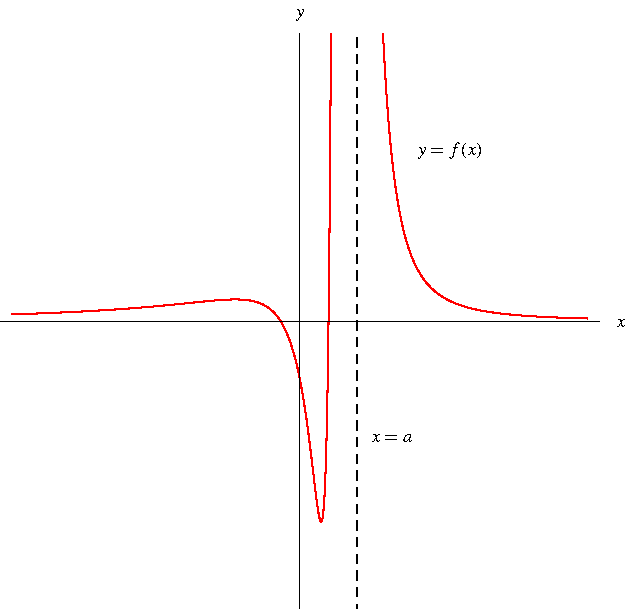
\includegraphics[height=4cm]{limits/pictures/02-02-posinf.pdf}%
\column{.6\textwidth}
\begin{itemize}
\item<2->  Other notation: $f(x) \rightarrow \infty $ as $x\rightarrow a$.
\item<3->  In such cases, the limit does not exist.
\item<4->  $\infty$ is not a number.  The notation $\lim\limits_{x\rightarrow a}f(x) = \infty$ expresses the particular way in which the limit doesn't exist.
\end{itemize}
\end{columns}
\end{frame}




\begin{frame}[t]
\begin{definition}[Infinite Limit]
Let $f$ be a function defined on both sides of $a$, except perhaps at $a$. Then
\[
\lim_{x\rightarrow a}f(x) = -\infty 
\]
means the values of $f(x)$ can be made arbitrarily negative by taking $x$ sufficiently close to $a$, but not equal to $a$.
\end{definition}
\begin{columns}[c]
\column{.4\textwidth}
\psset{xunit=0.15cm, yunit=0.15cm}
\begin{pspicture}(-10,-20)(16,7)
\psaxes[labels=none, ticks=none]{<->}(0,0)(-10,-20)(15,3)
\psplot[linecolor=red, plotpoints=1000]{1.39}{25}{x 1 x -1 add 2 exp div mul 0.8 mul x x mul 1 x -1 add 2 exp div mul 1.05 mul add 1 x -1 add 2 exp div 0.15 mul add -2 add -1 mul}
\psplot[linecolor=red, plotpoints=1000]{-10}{0.75}{x 1 x -1 add 2 exp div mul 0.8 mul x x mul 1 x -1 add 2 exp div mul 1.05 mul add 1 x -1 add 2 exp div 0.15 mul add -2 add -1 mul}
\psline[linestyle=dotted](1, -20)(1, 7)
\rput[l](1.5,4.5){$x=a$}
\rput(8,-5){$y=f(x)$}
\end{pspicture}%
%\ 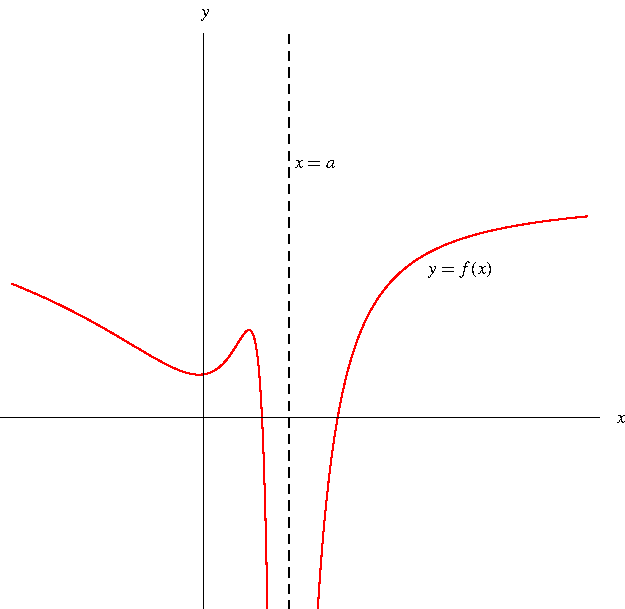
\includegraphics[height=4cm]{limits/pictures/02-02-neginf.pdf}%
\column{.6\textwidth}
\begin{itemize}
\item<2->  Here, by ``arbitrarily negative'' we mean the number is negative with large absolute value.
\item<3->  In such cases, the limit does not exist.
\item<4->  $-\infty$ is not a number.  The notation $\lim\limits_{x\rightarrow a}f(x) = -\infty$  expresses the particular way in which the limit doesn't exist.
\end{itemize}
\end{columns}
\end{frame}


\begin{frame}
There are similar definitions for one-sided limits:
\begin{tabular}{ccp{3cm}}
\begin{tabular}[c]{c}
\psset{xunit=0.13cm, yunit=0.13cm}
\begin{pspicture}(-6,-3)(15,16.5)
\psaxes[ticks=none, labels=none]{<->}(0,0)(-6,-3)(14,10)
\psplot[linecolor=red, plotpoints=1000]{-6}{6.65}{x x mul -0.6 mul x -0.9 mul add x x mul x mul 0.1 mul add 5.4 add x -7 add 2 exp div -2 add}
\psline[linestyle=dotted](7, -3)(7, 16.5)
\rput[tl](7.5, -1){$x=a$}
\end{pspicture} 
%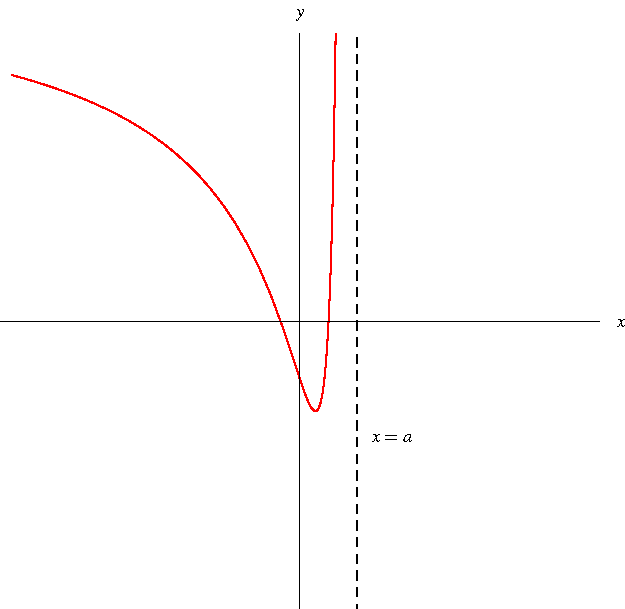
\includegraphics[height=3.2cm]{limits/pictures/02-02-posleft.pdf}
\end{tabular} &%
\begin{tabular}[c]{c}
\psset{xunit=0.13cm, yunit=0.13cm}
\begin{pspicture}(-6,-16.5)(14.5,3.5)
\psaxes[ticks=none, labels=none]{<->}(0,0)(-6,-10)(14,3)
\psplot[linecolor=red, plotpoints=1000]{-6}{6.65}{x x mul -0.6 mul x -0.9 mul add x x mul x mul 0.1 mul add 5.4 add x -7 add 2 exp div -2 add -1 mul}
\psline[linestyle=dotted](7, 3)(7, -16.5)
\rput[tl](7.5, -1){$x=a$}
\end{pspicture} 
%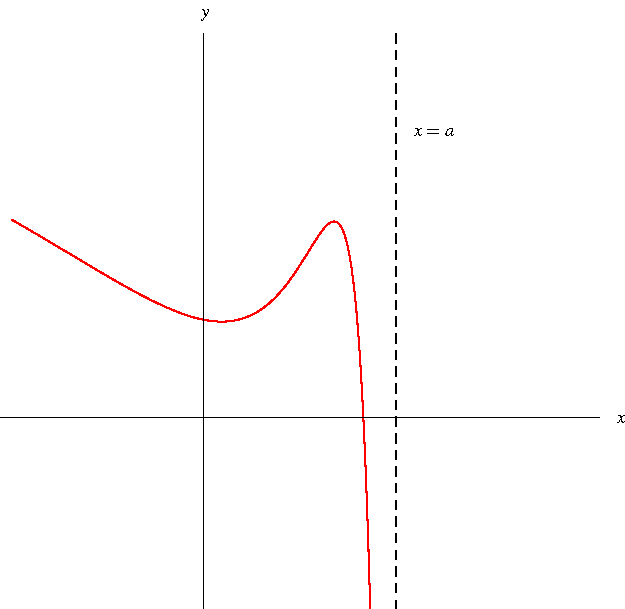
\includegraphics[height=3.2cm]{limits/pictures/02-02-negleft.pdf}
\end{tabular} &%
$x\rightarrow a^-$ means we only consider $x < a$.\\
$\lim\limits_{x\rightarrow a^-}f(x) = \infty$  & $\lim\limits_{x\rightarrow a^-} f(x) = -\infty$ & \\
\begin{tabular}[c]{c}
\psset{xunit=0.15cm, yunit=0.15cm}
\begin{pspicture}(-6,-5)(14.5,19.5)
\psaxes[ticks=none, labels=none]{<->}(0,0)(-6,-3)(14,14)
\psplot[linecolor=red, plotpoints=1000]{1.6}{17}{-2 x x mul x mul 0.1 mul x 2.7 mul add x x mul 1.2 mul add x -1 add 2 exp div add }
\psline[linestyle=dotted](1, -5)(1, 19.5)
\rput[tl](1.5, -3){$x=a$}
\end{pspicture} 
%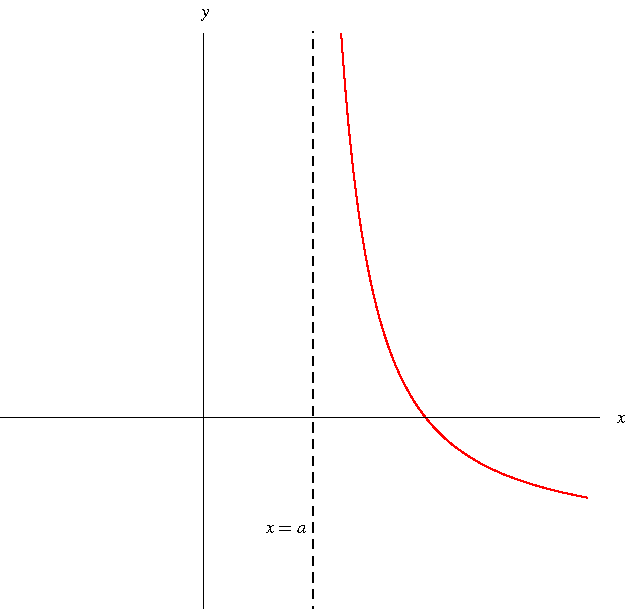
\includegraphics[height=3.2cm]{limits/pictures/02-02-posright.pdf}
\end{tabular} &%
\begin{tabular}[c]{c}
\psset{xunit=0.15cm, yunit=0.15cm}
\begin{pspicture}(-6,-19.5)(14.5,5.5) 
\psaxes[ticks=none, labels=none]{<->}(0,0)(-6,-14)(14,3)
\psplot[linecolor=red, plotpoints=1000]{1.6}{17}{-2 x x mul x mul 0.1 mul x 2.7 mul add x x mul 1.2 mul add x -1 add 2 exp div add -1 mul}
\psline[linestyle=dotted](1, 5)(1, -19.5)
\rput[tl](1.5, 3){$x=a$}
\end{pspicture} 
%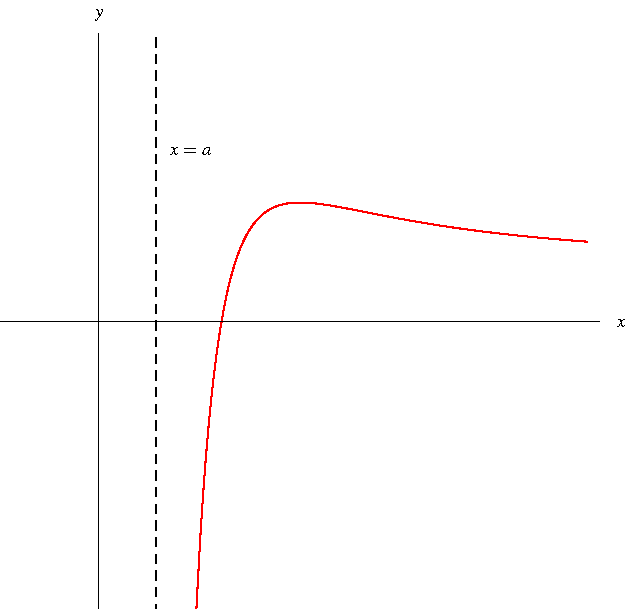
\includegraphics[height=3.2cm]{limits/pictures/02-02-negright.pdf}
\end{tabular} &%
$x\rightarrow a^+$ means we only consider $x > a$.\\
$\lim\limits_{x\rightarrow a^+}f(x) = \infty$  & $\lim\limits_{x\rightarrow a^+} f(x) = -\infty$ & \\
\end{tabular}
\end{frame}
% end module limits-infinite-def
